\documentclass[10pt,conference]{IEEEtran}
\usepackage[utf8]{inputenc}
\usepackage{amsmath}
\usepackage{amsfonts}
\usepackage{amssymb}
\usepackage{graphicx}
\usepackage{cleveref}
\usepackage{relsize}
\usepackage{bbm}

%% EDITING
\newcommand{\ie}{i.e.\ }
\newcommand{\eg}{e.g.\ }
\newcommand{\wrt}{w.r.t.\ }
\crefname{section}{\S}{\S\S}
\crefname{subsection}{\S}{\S\S}
\crefname{subsubsection}{\S}{\S\S}
\crefname{equation}{eq.}{}
\Crefname{equation}{Eq.}{}

%% MATHS

%% Probabilities
\newcommand{\Pro}[1]{\mathbb{P}\left[ #1 \right]}

%% Rounding, etc
\newcommand{\round}{\mathrm{Round}}
\newcommand{\pfp}{+_{\mathrm{fp}}}
\newcommand{\ceil}[1]{\lceil #1 \rceil}
\newcommand{\floor}[1]{\lfloor #1 \rfloor}
\newcommand{\intvl}[1]{\mathlarger{\left[\right.}  #1 \mathlarger{\left.\right]}}
\newcommand{\inv}{^{-1}}
\newcommand{\fintvl}[1][x]{\mathlarger{\lfloor}#1,#1\mathlarger{\rceil}}
\newcommand{\Err}{\mathcal{E}}
%% Sets
\newcommand{\F}{\mathbb{F}}
\newcommand{\R}{\mathbb{R}}
\newcommand{\N}{\mathbb{N}}
% Machine operation
\newcommand{\mop}{~\mathtt{op_m}~}
% Infinite-precision operation
\newcommand{\iop}{~\mathrm{op}~}
% Expectation
\newcommand{\Exp}[1]{\mathbb{E}\left[#1\right]}
% Indicator function
\newcommand{\one}{\mathbbm{1}}
%% General maths
\newcommand{\absv}[1]{\vert #1\vert}
\newcommand{\dt}{\frac{\partial}{\partial t}}



\title{A probabilistic approach to the accuracy and stability of numerical algorithms}
\author{George Constantinides and Fredrik Dahlqvist \hspace{10em}Rocco Salvia \\ Department of Electrical and Electronic Engineering\hspace{7em}University of Utah\\ Imperial College London\hspace{13em} }
\begin{document}
\maketitle

\begin{abstract}

\end{abstract}

\section{Introduction}

IEEE arithmetic \cite{ieee754} is traditionally modelled mathematically as follows \cite{higham2002accuracy}: if $x,y$ are two floating-point representable numbers and $\iop\in\{+,-,\times,\div\}$ is an infinite-precision arithmetic operation, then the floating-point precision implementation $\mop$ of $\iop$ must satisfy:
\begin{align}
x\mop y=(x\iop y)(1+\delta), \qquad\absv{\delta}\leq u\label{eq:traditional}
\end{align}
where $u$ is the unit roundoff for the given precision. \Cref{eq:traditional} says that the machine implementation of an arithmetic operation can make a relative error of size $\delta$ \emph{for some} $\delta\in\left[-u,u\right]$. The `\emph{for some}' is essential: this is a \emph{non-deterministic model}, we have no control whatsoever over which $\delta$ appears in \cref{eq:traditional}. This means that numerical analysis based on this model must consider \emph{all} possible values $\delta$, \ie numerical analysis based on \cref{eq:traditional} is fundamentally a \emph{worst-case analysis}. 

It also follows from the perspective of \cref{eq:traditional} that any program doing arithmetic is, in fact, a non-deterministic program. Moreover, since the output of such a program might very well turn out to be the input of another program doing arithmetic, one should also consider non-deterministic inputs. This is precisely what happens in practice with tools for numerical analysis like the recent Daisy \cite{darulova2018daisy} or FPTaylor \cite{solovyev2018rigorous} which require for each variable of the program a range of possible values in order to perform a worst-case analysis.

However, for a wide variety of programs  it makes sense to assume that the inputs are \emph{probabilistic} rather than non-deterministic; that is to say we have some statistical model of the inputs of the program. This situation is in fact incredibly common. The inputs of one numerical routine are frequently generated randomly by another numerical routine, for example in a gradient descent optimization, a Bayesian inference algorithm, or a stochastic ray tracing algorithm. Similarly, sensors on a cyber-physical system can feed analog signals which are very well modelled statistically, to a numerical program processing these signals. 

If the inputs of a program have a known distribution, then it becomes possible, at least in principle, to ask the question: \textit{How likely are the inputs generating the worst-case rounding errors obtained from the non-deterministic model of \cref{eq:traditional}?} Typically, these inputs will occur very infrequently, and in this respect the non-deterministic model can be overly pessimistic since worst-case behaviours might be such rare events that they are never encountered in practice. 

In this paper we will explore a quantitative model which formally looks very similar to \cref{eq:traditional}, namely
\begin{align}
x\mop y=(x\iop y)(1+\delta), \qquad\delta\sim dist \label{eq:probabilistic}
\end{align}
but now $\delta$ is \emph{sampled} from $dist$, a probability distribution whose support is $\left[-u,u\right]$. In other words we move from a non-deterministic model of rounding errors to a \emph{probabilistic} model of rounding errors. This model will allow us to formalise and answer questions like: \textit{What is the distribution of outputs when rounding errors are taken into account?} \textit{What is the average rounding error?} \textit{What is the worst-case error with $99.9\%$ accuracy?}

As was mentioned above, model \eqref{eq:traditional} amounts to saying that any numerical program is a non-deterministic program. Completely analogously, in the perspective of \cref{eq:probabilistic} every numerical program is a \emph{probabilistic program}, that is to say a program which admits sampling as a native instruction. The study of probabilistic programs goes back to Kozen \cite{K81c} which modelled simple \texttt{while} programs containing an \emph{explicit} sampling instruction \texttt{random()}. In our setting any numerical program becomes a probabilistic program via an \emph{implicit} sampling operation which takes place whenever an arithmetic operation is performed. This implicit sampling is the only difference with the standard setting of \cite{K81c}, and we will otherwise understand how programs process randomness by following the framework laid out in \cite{K81c}. The study of probabilistic programs has recently witnessed a resurgence of interest driven by new applications in machine learning and statistical analysis of large datasets. As far as we know this is the first attempt to bring the techniques of probabilistic program analysis to bear on the problem of numerical accuracy.

The probabilistic model of \cref{eq:probabilistic} is not new, it can be traced back to von Neumann and Goldstine \cite{von1947numerical} and is very similar to the so-called Monte-Carlo arithmetic of \cite{parker1997monte}. More recently, the model of \cref{eq:probabilistic} has been investigated by Higham \cite{higham2019new}
and Ipsen \cite{ipsen2019probabilistic}. Interestingly, because \cite{higham2019new} and \cite{ipsen2019probabilistic} are interested in large-dimensional problems, neither work needs to explicitly specify the distribution $dist$ in \cref{eq:probabilistic}. Instead, \cite{higham2019new} requires that each sample from $dist$ be independent and that $\Exp{\delta}=0$, whilst \cite{ipsen2019probabilistic} just requires that $\Exp{\delta}=0$. By using concentration of measure inequalities the authors then obtain probabilistic bounds which are independent of any particular choice of distribution. 
These bounds however are only useful for large programs. Here we will derive a principled distribution $dist$ for the relative error $\delta$ in order to apply the probabilistic model \cref{eq:probabilistic} to small to medium programs, in particular some benchmark from the literature on verification of numerical programs.

\section{Two probabilistic models of rounding errors}

In order to use the probabilistic model given by \cref{eq:probabilistic} we must specify the distribution $dist$ of the random variable $\delta$. In this section we will show how to derive the distribution of rounding errors from first principles. This will yield a distribution which is computable for low precisions (\eg half-precision and lower) but becomes prohibitively expensive computationally for single- and double-precision. We will then show that very often the rounding error distribution can be approximated remarkably well by a simple distribution which we shall call the \emph{typical distribution}. The quality of this approximation increases with the working precision and we thus derive both an exact, computable model of rounding errors for low-precisions, and a simple but good approximating model of rounding errors for high-precisions.

\subsection{The exact rounding error distribution}\label{subsec:error_dist}

Conceptually, the key to our approach is to model the rounding operation probabilistically, \ie as an operation which adds a probabilistic relative error via
\begin{align}
x \longrightarrow x(1+\delta)\qquad \delta\sim dist.\label{eq:rounding}
\end{align}
Since each IEEE arithmetic operation can be understood as implicitly performing a rounding operation on the corresponding infinite-precision operation, the probabilistic rounding above naturally yields \cref{eq:probabilistic}. The key is thus to find a good candidate for the distribution $dist$ governing probabilistic rounding.

As discussed in the introduction, we consider numerical programs as probabilistic programs. In particular, all inputs come with probability distributions, and we should consider the variable $x$ in \cref{eq:rounding} as a sample from a real random variable $X$ with known probability distribution $\mathbb{P}$. It is then completely natural to require that:
\[
\frac{X-\round(X)}{X}~\sim~dist
\]
\ie $dist$ describes the distribution of the actual, deterministic rounding error of samples drawn from $X$. We will now explicitly compute $dist$. First we introduce some convenient notation. We define
\begin{align*}
\ceil{x}&\stackrel{\triangle}{=}\sup\{z\in\R\mid \round(z)=\round(x)\}\\
\floor{x}&\stackrel{\triangle}{=}\inf\{z\in\R\mid \round(z)=\round(x)\}.
\end{align*}
Whether $\ceil{x}$ is the maximal real which rounds to the same value as $x$, or just the supremum of this set, will in general depend both on $x$ and on the rounding convention, and similarly for $\floor{x}$. We also define the sets 
\[
\fintvl\stackrel{\triangle}{=}\left\{z\in\R\mid \round(z)=\round(x)\right\}
\]  
In particular if $z$ is a floating-point representable number -- notation $z\in\F$ -- then $\fintvl[z]$ is the collection of all reals rounding to $z$.

We choose to express the distribution $dist$ of relative errors in multiples of the unit roundoff $u$. This choice is arbitrary, but it allows us to normalize the distribution since the absolute value of the relative error is strictly bounded by $u$. In other words, we express the relative error as a distribution on $[-1,1]$ rather than $[-u,u]$. In order to compute the density function of $dist$ we proceed in the standard way by first computing the cumulative distribution function $c(t)$ and then taking its derivative. We therefore start by computing
\begin{align*}
c(t)\stackrel{\triangle}{=}&~\Pro{\frac{X-\widehat{X}}{X}\leq tu}\\
=&~\Pro{~\bigvee_{z\in\F}\left(\frac{X-z}{X}\leq tu\wedge X\in \fintvl[z]\right)}
\end{align*}
We now need to consider three special cases:
\begin{enumerate}
\item If $X\in \fintvl[0]$ then $\frac{X-\widehat{X}}{X}=1$ and thus (since $tu<1$):
\begin{align}\label{eq:cdfnot0}
\Pro{\frac{X-0}{X}\leq tu\wedge X\in \fintvl[0]}=0
\end{align}
\item If $X\in \fintvl[-\infty]$ then $\frac{X-\widehat{X}}{X}=\infty$ and thus 
\begin{align}\label{eq:cdfnotminf}
\Pro{\frac{X+\infty}{X}\leq tu\wedge X\in \fintvl[-\infty]}=0
\end{align}
\item Finally, if $X\in \fintvl[\infty]$ then $\frac{X-\widehat{X}}{X}=-\infty$ and thus 
\begin{align}\label{eq:cdfpinf}
\hspace{-3em}\Pro{\frac{X-\infty}{X}\leq tu\wedge X\in \fintvl[\infty]}=\Pro{X\in \fintvl[\infty]}
\end{align}
\end{enumerate}
Using the fact that \eqref{eq:cdfnot0}-\eqref{eq:cdfpinf} yield expressions which are independent of $t$ we get the density
\begin{align*}
d(t)=&\dt c(t)\\
=&\dt\sum_{z\in\F\setminus\{-\infty,0,\infty\}}\hspace{-1em}\Pro{\frac{X-z}{X}\leq tu\wedge X\in \fintvl[z]}\\
=& \sum_{z\in\F^-\setminus\{-\infty,0\}}\dt\Pro{\frac{z}{1-tu}\geq X\wedge X\in \fintvl[z]}+\\
&\sum_{z\in\F^+\setminus\{0,\infty\}}\dt\Pro{\frac{z}{1-tu}\leq X \wedge X\in \fintvl[z]}
\end{align*}
where $\F^+$ and $\F^-$ denote the positive (resp. negative) floating-point representable numbers.
Suppose now that $X$ is described by a probability density function $f:\R\to\R$, we then get:
\begin{align}
d(t)
=&\hspace{-1ex}\sum_{z\in\F^-\setminus\{-\infty,0\}}\dt\one_{\fintvl[z]}\left(\frac{z}{1-tu}\right) \int^{\frac{z}{1-tu}}_{\floor{z}} f(s)~ds+\nonumber 
\\
&\sum_{z\in\F^+\setminus\{0,\infty\}}\dt\one_{\fintvl[z]}\left(\frac{z}{1-tu}\right) \int^{\ceil{z}}_{\frac{z}{1-tu}} f(s)~ds\nonumber 
\\
=&\hspace{-2ex}\sum_{z\in\F^-\setminus\{-\infty,0\}}\hspace{-1ex}\one_{\fintvl[z]}\hspace{-4pt}\left(\frac{z}{1-tu}\right) f\hspace{-3pt}\left(\frac{z}{1-tu}\right) \frac{-uz}{(1-tu)^2}\nonumber
\\
& +\hspace{-2ex}\sum_{z\in\F^+\setminus\{0.\infty\}}\hspace{-2ex}\one_{\fintvl[z]}\hspace{-4pt}\left(\frac{z}{1-tu}\right) f\hspace{-3pt}\left(\frac{z}{1-tu}\right) \frac{uz}{(1-tu)^2}\nonumber 
\\
=&\hspace{-2ex}\sum_{z\in\F\setminus\{-\infty,0,\infty\}}\hspace{-2ex}\one_{\fintvl[z]}\hspace{-4pt}\left(\frac{z}{1-tu}\right) f\hspace{-3pt}\left(\frac{z}{1-tu}\right) \frac{u\absv{z}}{(1-tu)^2}\label{eq:errorDensity}
\end{align}
where $\one_{A}(x)$ is the usual indicator function which returns 1 if $x\in A$ and 0 otherwise. For low precisions, that is to say up to half-precision (5 bits exponent, 10 bits mantissa), it is perfectly possible to explicitly go through all floating point numbers and compute the density of the rounding error distribution $dist$ by using \cref{eq:errorDensity}. However this rapidly becomes too computationally expensive for higher-precision (since the number of floating-point representable numbers grows exponentially).





\subsection{The typical rounding error distribution}
Interestingly, when computing the error density \cref{eq:errorDensity} for a wide variety of well-known input distribution, one very often obtains more or less the same curve. This phenomenon is illustrated in \cref{fig:errdist} where the half-precision error density computed via \cref{eq:errorDensity} is displayed for uniform distributions over $\left[-10,10\right]$ and $\left[0,1\right]$ and for normal distributions with parameters $\mu=0,\sigma=2$ and $\mu=2,\sigma=10$ respectively. The reader will notice immediately that all the curves are nearly identical.

\vspace{-1em}
\begin{figure}[h!]
\hspace{-3em}
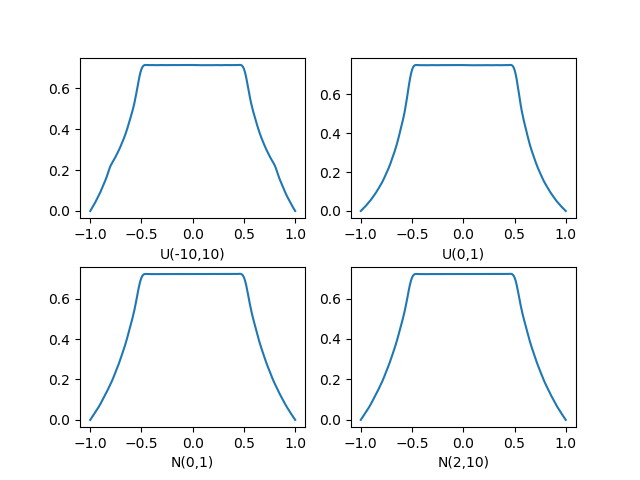
\includegraphics[scale=0.65]{pics/several_examples}
\caption{Half-precision relative error distribution for four typical input distributions}
\label{fig:errdist}
\end{figure}

In this section we will sketch how, under some regularity assumptions about the input distribution, the error density of \cref{eq:errorDensity} can be approximated by a simple, piecewise polynomial curve which we shall call the \emph{typical error distribution}. The precise mathematical derivation of this curve being relatively long, we refer the reader to XXX for the full details. Here we will simply specify conditions under which the error distribution given by \cref{eq:errorDensity} is close to the typical distribution. The key observations which we shall make are that (a) the quality of the approximation increases with the working precision (henceforth $p$), and (b) the likelihood of the assumptions being satisfied also increases with $p$.

Let $z(e,s,k)$ denote the floating-point representable real with exponent $e$, sign $(-1)^s$ and mantissa $k$, and let $e_{min}$ and $e_{max}$ denote the smallest and largest exponents respectively. Given a $t\in \left[-1,1\right]$, one can show that the mantissas such that
\begin{align}
\one_{\fintvl[z(e,s,k)]}\left(\frac{z(e,s,k)}{1-tu}\right)=1\label{eq:membership}
\end{align}
are given by 
\begin{align}
k\leq 2^p\left(\frac{1}{\absv{t}}-1\right)-\frac{1}{2}\label{eq:mantissas}
\end{align}
Note that for $t\in \left[-\frac{1}{2},\frac{1}{2}\right]$ \cref{eq:mantissas} always holds, \ie all mantissa are compatible with \cref{eq:membership}.
We can now specify our assumptions.

\noindent \textbf{Assumption 0.} The probability density function is constant at the scale of the intervals between floating point numbers, \ie
\begin{align*}
\Pro{\round(x)=z}
&=\int_{\floor{z}}^{\ceil{z}} f(x)~dx 
\\
&\approx f\left(\frac{z}{1-tu}\right)(\ceil{z}-\floor{z})
\end{align*}
for all values of $t$ such that \cref{eq:membership} holds.

\noindent  \textbf{Assumption 1.} Writing $z(s,k)$ for $z(e_{min},s,k)$ assume that:
\[
\sum_{\substack{0\leq k<2^p\\ s\in\{0,1\}}}\hspace{-4pt}\one_{\fintvl[z]}\hspace{-4pt}\left(\frac{z(s,k)}{1-tu}\right)f\hspace{-3pt}\left(\frac{z(s,k)}{1-tu}\right)\hspace{-2pt}(\ceil{z(s,k)}-\floor{z(s,k)})\approx 0
\]
and similarly for $z(s,k)=z(e_{max},s,k)$.
Under Assumption 0, this condition says that the probability under $f$ of sampling a number whose rounding has exponent $e_{min}$ or $e_{max}$ is close to zero. This condition is certainly met for the distributions of \cref{fig:errdist} and half-precision.

\noindent \textbf{Assumption 2.} Given $t\in\left[-1,1\right]$, for every $k$ satisfying \cref{eq:mantissas} we assume
\[
\sum_{\substack{e_{min}<e<e_{max}\\ s\in\{0,1\}}}f\hspace{-2pt}\left(\frac{z(e,s,k)}{1-tu}\right)(\ceil{z(e,s,k)}-\floor{z(e,s,k)})\approx \frac{1}{2^p}
\]
Under assumption 0, this condition means that when rounding a sample drawn from the distribution $f$, all mantissas are equally likely.

Under assumptions 0-2 one can show that for $t\in\left[-\frac{1}{2},\frac{1}{2}\right]$
\begin{align}
d(t)\approx\frac{1}{2^p(1-tu)^2}\left(\frac{2}{3}+\frac{3(2^{p}-1)}{4}\right)\label{eq:pdfmiddle}
\end{align}
Similarly, under assumptions 0-2 one has for $\absv{t}>\frac{1}{2}$:
\begin{align}
d(t)\approx\frac{1}{2^p(1-tu)^2}& \left(\frac{2}{3}+\frac{1}{2}\floor{2^p(\frac{1}{t}-1)-\frac{1}{2}}+\right. \nonumber 
\\
&\left.\frac{1}{2^{p+2}}(\floor{2^p(\frac{1}{t}-1)+\frac{1}{2}})^2\right)\label{eq:pdfwings}
\end{align}
where $\floor{2^p(\frac{1}{t}-1)+\frac{1}{2}}$ here denotes the usual floor function.
Combining \cref{eq:pdfmiddle} and \cref{eq:pdfwings} we get under assumptions 0-2 that as $p\to\infty$ the error density $d(t)$ is well approximated by the \emph{typical density}:
\begin{align}
d_{typ}(t)=\begin{cases}
\frac{3}{4}&\absv{t}\leq\frac{1}{2}
\\
\frac{1}{2}\left(\frac{1}{t}-1\right)+\frac{1}{4}\left(\frac{1}{t}-1\right)^2 & \absv{t}>\frac{1}{2}
\end{cases}\label{eq:typicalpdf}
\end{align} 
which is represented in \cref{fig:typical} and is clearly a good approximation of the exact densities of \cref{fig:errdist}.
\begin{figure}[ht!]
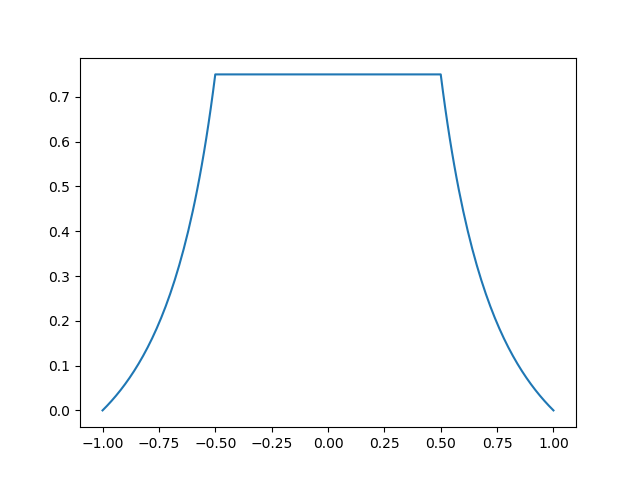
\includegraphics[scale=0.55]{pics/typical_dist}
\caption{Typical distribution of rounding errors (in unit roundoffs)}
\label{fig:typical}
\end{figure}


\textbf{Remark:}
A remark to the effect that assumptions 0-2 are increasingly likely to be met as $p\to\infty$.



\section{Probabilistic interpretation of simple expressions}

\subsection{A simple syntax}

The numerical expressions which we will investigate are given by the following simple grammar.
\begin{align*}
&\textbf{Terms: }  
\\
& \tt t::= r \mid x_i \mid t\mop t \qquad \mathtt{r}\in\F, \mathtt{i}\in\N, \mop\hspace{-1ex}\in\{+.-,\times,\div\}
\\
&\textbf{Tests: } 
\\
& \tt b::= t < r \mid t > r \mid t == r  \qquad \mathtt{r}\in\F
\\
&\textbf{Expressions:}
\\ 
&\tt p::= skip \mid \mathtt{x_i:=t}\mid \mathtt{p~;~p} \mid if~b~then~p~else~p
\end{align*}

For every expression $\mathtt{p}$, we consider the list $\{\mathtt{x_1,\ldots,x_n}\}$ of variables appearing in $\mathtt{p}$. We view all variables as public variables and we will associate to each of them a real random variable $X_i, 1\leq i\leq n$ modelling its (probabilistic) state. We will call this data the \emph{probabilistic context} and denote it $\{\mathtt{x_1}\sim X_1,\ldots,\mathtt{x_n}\sim X_n\}$.  We also assume an exponent range $e_{min}, e_{max}$ and a precision level $p$ throughout.

\subsection{Random variable arithmetic}

It is relatively well-known that arithmetic operations on random variables which posses a density function (\wrt the Lebesgue measure) translate into operations on these densities \cite{springer1979algebra}. In particular the density of the sum of two random variable is given by the convolution of the densities. In more detail one has the following correspondence:
\begin{align}
X+Y&\sim f_X\oplus f_Y(t)=\int_{-\infty}^{\infty} f_X(x)f_Y(t-x)~dx\label{eq:pdfplus}\\
X-Y&\sim f_X\ominus f_Y(t)=\int_{-\infty}^{\infty} f_X(x)f_Y(x-t)~dx\label{eq:pdfminus}\\
X\times Y&\sim f_X\otimes f_Y(t)=\int_{-\infty}^{\infty} \frac{1}{\absv{x}}f_X(x)f_Y\left(\frac{t}{x}\right)dx\label{eq:pdftimes}\\
X\div Y&\sim f_X\oslash f_Y(t)=\int_{-\infty}^{\infty} \absv{x}f_\mu(x)f_\nu(tx)dx\label{eq:pdfdiv}
\end{align}
Similarly, addition and multiplication by a scalar correspond to
\begin{align*}
\alpha+X&\sim (\alpha\oplus f_X)(t)=f(t+\alpha)\\
\alpha X&\sim (\alpha\otimes f_X)(t)=\alpha f(\alpha t)
\end{align*}

\subsection{Probabilistic interpretation}

For any random variable $X$ with density $f_X$, we will define the \emph{error of $X$} -- notation $\Err(X)$ -- as the random variable $\frac{X-\widehat{X}}{X}$ whose density is given by \cref{eq:errorDensity}.

\subsubsection{Input quantization} Given a probabilistic context, the first question is to decide whether we need to model an initial quantization. This would correspond, for example, to modelling the quantization of an analog input (\eg a sensor) or of an input generated at a higher precision level (\eg a routine at half-precision level receiving input in double-precision). If we choose to model this step, then we need to add a probabilistic error term to each input, this is achieved by the probabilistic quantization
\[
X\longrightarrow X(1+\Err(X))
\] 

\subsubsection{Terms} will be modelled as random variables using the following inductive definition:
\begin{align*}
model(\mathtt{r})&= r\text{, the constant r.v.}\\
model(\mathtt{x_i})&= X_i\\
model(\mathtt{t_1\mop t_2})&=\left(model(\mathtt{t_1})\iop model(\mathtt{t_2})\right)\cdot \\
& \hspace{12pt}\left(1+\Err(model(\mathtt{t_1})\iop model(\mathtt{t_2}))\right)
\end{align*}

Note how we model the arithmetic operations in accordance with the fundamental model of \cref{eq:probabilistic}: we first compute the random variable $model(\mathtt{t_1})\iop model(\mathtt{t_2})$ which corresponds to the infinite-precision operation, and we then add a probabilistic error term whose distribution is computed from the distribution of $model(\mathtt{t_1}\iop\mathtt{t_2})$ itself.

\subsubsection{Tests} correspond to the obvious subset of $\R^n$ generated by the comparisons. Thus if $\mathtt{t(x_1,\ldots,x_n)}$ is a term on $n$ variables 
\[
model(\mathtt{t<r})=\{(x_1,\ldots,x_n)\in\R^n\mid \mathtt{t}(x_1,\ldots,x_n)<r\}
\]
and similarly for $\mathtt{t>r}$ and $\mathtt{t==r}$. Note that terms are not viewed as probabilistic in this context, simply as a way of specifying a subset of $\R^n$.

\subsubsection{Expressions} will be modelled as operations sending $n$ random variables (one for each variable) to $n$ random variables. In effect, updating the probabilistic context.

\begin{align*}
model(\mathtt{skip})(X_1,\ldots,X_n)&=(X_1,\ldots,X_n)\\
model(\mathtt{x_i}:=t)(X_1,\ldots,X_n)&=(X_1,, X_{i-1},model(\mathtt{t}),X_{i+1},\ldots,X_n)\\
model(\mathtt{p_1~;~p_2})(X_1,\ldots,X_n)&=model(\mathtt{p_2})(model(\mathtt{p_1})(X_1,\ldots,X_n))
\end{align*}


\section{Experimental results}

\subsection{Stability: ray tracing via the slabs method}

\bibliographystyle{plain}
\bibliography{bib/constantinides-dahlqvist}

\end{document}